\documentclass{article}
\usepackage{amsmath}
\usepackage{xcolor}
\usepackage{gensymb}
\usepackage{ragged2e}
\usepackage{graphicx}
\usepackage{gensymb}
\usepackage{mathtools}
\newcommand{\mydet}[1]{\ensuremath{\begin{vmatrix}#1\end{vmatrix}}}
\providecommand{\brak}[1]{\ensuremath{\left(#1\right)}}
\providecommand{\norm}[1]{\left\lVert#1\right\rVert}
\newcommand{\solution}{\noindent \textbf{Solution: }}
\newcommand{\myvec}[1]{\ensuremath{\begin{pmatrix}#1\end{pmatrix}}}
\let\vec\mathbf
\begin{document}
\begin{center}
        \textbf\large{CHAPTER-11 \\ TRIANGLES}
\end{center}
\section{Exercise 11.2}
Q5.Construct a right triangle whose base is 12$cm$ and sum of its hypotenuse and other side is 18$cm$ \\
\textbf{Solution:}
Let $\vec{A}$,$\vec{B}$ and $\vec{C}$ are the vertices of the right triangle with coordinates.
Given $BC=12cm$(base).So the coordinates of vertices $\vec{B}$,$\vec{C}$ are:
\begin{align}
{
\vec{B} =\myvec{0\\0},\vec{C} =\myvec{a\\0}
}
\end{align}
Also given $\angle{B}=90\degree$, so by finding the coordinates of the other side we can form a required triangle. \\
 The input parameters for this construction are
 \begin{table}[h]
   \centering
   \begin{tabular}{|c|c|c|}
  \hline
  \textbf{Symbol}&\textbf{Value}&\textbf{Description}\\
  \hline
  $a$ & 12 & $BC$\\
  \hline
  $\theta$ & 90$\degree{}$ & $\angle{B}$ in $\triangle ABC$ \\
  \hline
  $k$ & 18 & $AB+AC$ i.e $b+c$ \\
  \hline 
  $\vec{e_2}$ & $\myvec{0\\1\\}$ & Basis vector\\
  \hline   
\end{tabular}\\

   \caption{Parameters}
   \label{tab:Table1}
\end{table}\\
Caluclating Other Coordinate:
  \begin{align}
	  \vec{A} = c\myvec{\cos{\theta} \\ \sin{\theta}}
   \end{align}
We know that\\
\begin{align}  
	c = \frac{1}{2(1-\frac{a\cos{\theta}}{k})}\vec{e}_2^{\top}\myvec{1 & 1\\-1 & 1}\myvec{\frac{a^2}{k}\\k}
     \end{align}
  \begin{align}
	  c = 5
  \end{align}  
The vertices of $\triangle ABC$ are \\
\begin{align}
\vec{A} = 5\myvec{\cos 90\degree\\\sin 90\degree}
  = \myvec{0\\5}
\end{align}
\begin{align}
 \vec{B} = \myvec{0\\0}
\end{align}
\begin{align}
 \vec{C} = \myvec{12\\0}
 \end{align}        
Construction: 
\begin{figure}[h]
 \begin{center}
  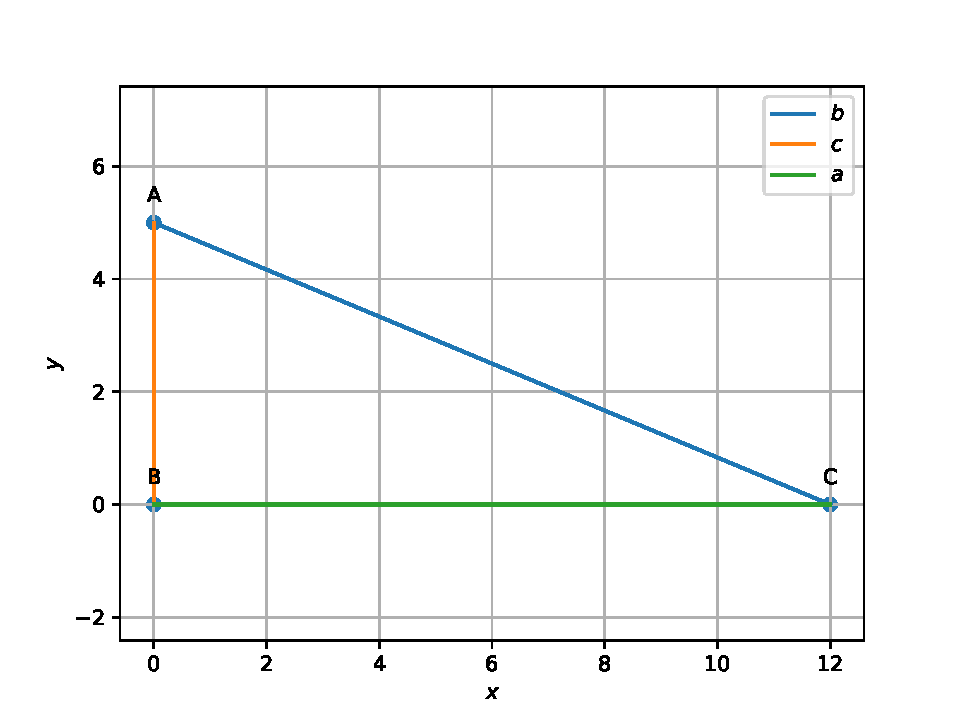
\includegraphics[width=\columnwidth]{figs.pdf}
 \end{center}
 \caption{Triangle ABC}
 \label{fig:Fig1}
\end{figure}
\end{document}
